\documentclass{gajewski}

\bibliographystyle{IEEEtran}

%%%%%%%%%%%%%%%%%
% Document variables
%%%%%%%%%%%%%%%%%
\docDate{ \today }
\docID{Present Cipher ("Pure Testing") - with communication channel with PC}
\docRevision{0.2}
\docStatus{Draft}
\docTitle{\mbox{Present Cipher ("Pure Testing") -} \mbox{with communication channel with PC}} 
\docTitleShort{Present Cipher ("Pure Testing")...}
\authorName{\mbox{Krzysztof Gajewski} \\ and opencores.org}
\authorURL{www.opencores.org}
\authorAddress{\mbox{}}
\authorEmail{gajos@opencores.org}

\revisionList{ 
0.1 & all & 2014/05/01 & First draft & K. Gajewski \\
0.2 & all & 2014/09/16 & Some small corrections with the text, typos, etc. & K. Gajewski \\
}

\begin{document}

\maketitle

\newpage

\revisionTable

\newpage

\tableofcontents
\newpage

\section{Introduction}

Present is "ultra-lightweight" block cipher developed by A. Bogdanov et al. and proposed in 2007 \cite{PRESENT}. It uses 64 bit data block and 80 bit or 128 bit key.
This cipher consists of 32 rounds, during which: 
\begin{itemize}
    \item round key is added to plaintext
    \item plaintext goues through sBoxes (substitution boxes)
    \item plaintext after sBoxes goes through pLayer (permutation layer)
    \item round key is updated
\end{itemize}
After that, ciphertext feeds out the output. Briefly algorithm was shown in Fig. \ref{pAlgorithm}. 
\begin{figure}[!ht]%
    \begin{center}
    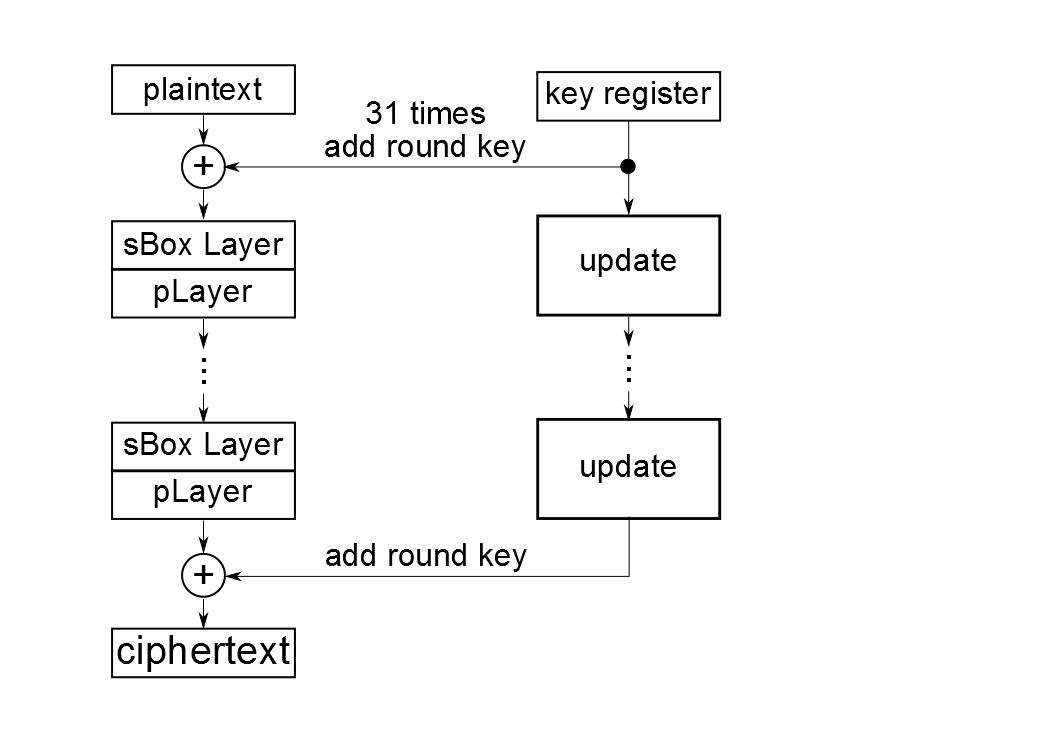
\includegraphics[width=0.66\textwidth]{img/presentAlgorithm.png}
    \caption{%
        Briefly block scheme of the PRESENT block cipher
     }%
    \label{pAlgorithm}
    \end{center}
 \end{figure}
More informations about FPGA Present core can be found in "Pure" subfolder.
In this project Present block cipher works with 80 bit key. It was attached by shifting registers to RS-232 core developed by Digilent\textsuperscript{\textregistered} to enable communication with PC. Target was Xilinx\textsuperscript{\textregistered} Spartan 3E XC3S500E \cite{Spartan} on Spartan 3E  Starter Board \cite{Digilent} made by Digilent\textsuperscript{\textregistered}.

\newpage 

\section{Interface}

Top level component of the Present Pure Testing was shown in Fig. \ref{ptest}. The number of inputs and outputs was limited due to RS-232 component in communication interface. All inputs and outputs are synchronous except \texttt{reset} signal and sampled at rising edge of clock. All signals are \texttt{STD\_LOGIC}.
\begin{figure}[!ht]%
    \begin{center}
    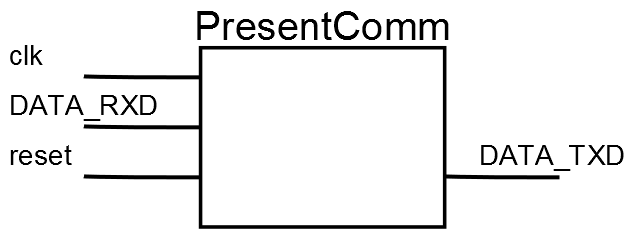
\includegraphics[width=0.5\textwidth]{img/PresentPureTesting.png}
    \caption{%
        Top level component of the Present Pure Testing 
     }%
    \label{ptest}
    \end{center}
 \end{figure}

\begin{tabularx}{\textwidth}{|p{30mm}|p{11mm}|p{11mm}|X|}
  \hline \bf{Signal name} & \bf{Width} & \bf{In/Out} & \bf{Description}\\ 
  \hline \texttt{clk} & 1  &  in  & clock signal for the component. \\ 
  \hline \texttt{DATA\_RXD} & 1 & in & input data signal. \\
  \hline \texttt{reset}	& 1  &  in  &  \emph{asynchronous} reset signal.\\ 
  \hline \texttt{DATA\_TXD} & 1 &  out  & output data signal.	\\ 
  \hline
\end{tabularx}
\captionof{table}{Input/Output signals of the Present component}

\newpage

\section{Internal structure and state machine workflow}

Internal datapath between components was shown in fig. \ref{pinside}. All control signals, \texttt{clk} and \texttt{reset} was omitted for clearance. In these schamatic \texttt{keyReg}, \texttt{textReg} and \texttt{outReg} are shift registers enabling conversion of the serial input/output data into parallel data. They are respectively:
\begin{itemize}
    \item \texttt{keyReg} - shift register for the key,
    \item \texttt{textReg} - shift register for the text to be encoded,
    \item \texttt{outReg} - shift register for the output data to be sendend by RS232.
\end{itemize}
\texttt{present} - is the crypto core. It was described in \texttt{./Present/doc/present\_pure.pdf} file ("Present" subproject documentation). \texttt{RS232} is the serial communication core developed by Digilent\textsuperscript{\textregistered} responsible for the communication with PC computer.
\texttt{SM} is state machine which manage communication with PC and data conversion before and after data encoding in \texttt{present} component.

\begin{figure}[!ht]%
    \begin{center}
    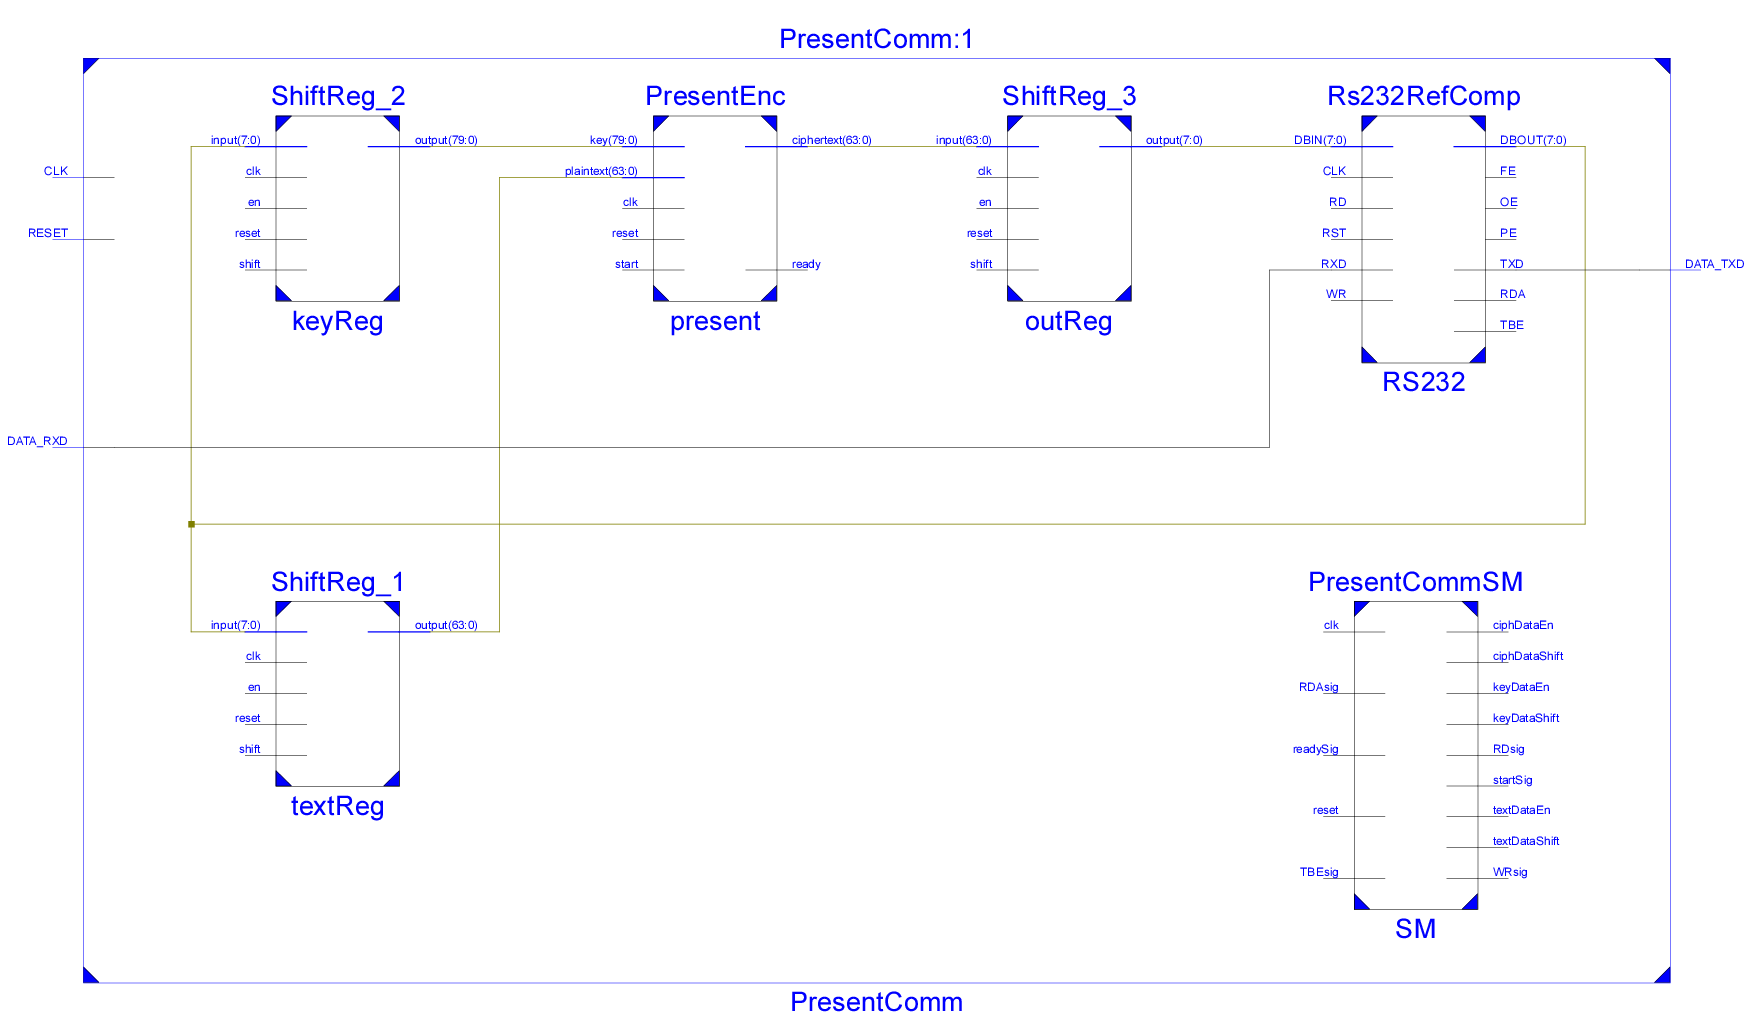
\includegraphics[width=0.95\textwidth]{img/PresentCommInside.png}
    \caption{%
        Internal structure of the Present core with communication environment. 
     }%
    \label{pinside}
    \end{center}
 \end{figure}

State machine states and transition between them was shown in fig. \ref{presentCommSM}.

\begin{figure}[!ht]%
    \begin{center}
    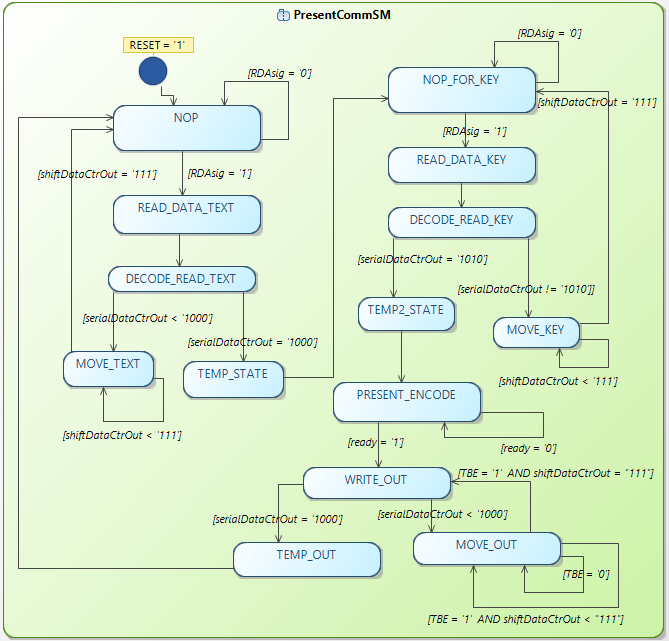
\includegraphics[width=0.95\textwidth]{img/PresentCommSM.png}
    \caption{%
        State machine of the Present cipher with added communication component
     }%
    \label{presentCommSM}
    \end{center}
 \end{figure}


State machine consist of following states, which are briefly explained:

\begin{itemize}
    \item \texttt{NOP} - this is the initial state of the state machine. It is set up after resetting the system. If any data appear in the RS-232 input (\texttt{RDAsig = '1'}), this state will be changed.
    \item \texttt{READ\_DATA\_TEXT} / \texttt{READ\_DATA\_KEY} - These states inform the RS-232 component that input data was read (by write enable in \texttt{keyReg} register). 
    \item \texttt{DECODE\_READ\_TEXT} / \texttt{DECODE\_READ\_KEY}- In these states the number of performed data reading iterations are checked. Because one RS-232 packet was set to 8 bytes - 8 iterations need to be ferformed for reading full 64 bit text data input (10 iterations for reading full 80 bit key data input).
    \item \texttt{TEMP\_STATE} / \texttt{TEMP2\_STATE} / \texttt{TEMP\_OUT} - Here the counter is prepared for key reading / encoding / next "encoding session".
    \item \texttt{MOVE\_TEXT} / \texttt{MOVE\_KEY} / - Due to serial data in RS-232 component are stored in 8 bit register, they need to be shifted in appropriate place in given shift registers. It is performed by 8 shifts made in 8 clock cycles.
    \item \texttt{NOP\_FOR\_KEY} - Kind of \texttt{NOP} or wait state until 'key' data will arrive.
    \item \texttt{PRESENT\_ENCODE} - In this state Present encoding is performed. This state is active until Present component informs about ending of the encoding process (\texttt{readySig = '1'}).
    \item \texttt{WRITE\_OUT} - state responsible for immediate sending encoded data. It is performed as many number as 64 bits of encoded data will be sent by the RS-232 component to the PC (similarly to "\texttt{DECODE...}" states). 
    \item \texttt{MOVE\_OUT} - it is similar state to the previous \texttt{MOVE...} states, but here additionally state machine must wait until output data buffer will be prepared for next data which have to be sended.
\end{itemize}
No "lost data" checking, and data correction protocol was performed. It was assumed "ideal channel" for communication. Some states could be "merged" into one state but it will involve more expanded control logic.

\newpage

\section{FPGA implementations}

The  component  has been verified on a Xilinx\textsuperscript{\textregistered} Spartan 3E XC3S500E FPGA in FG320 package and synthesized  with  Xilinx  ISE  14.2. It was also implemented and practically tested on Spartan 3E Starter Board made by Digilent\textsuperscript{\textregistered}. Appropriate setup files was prepared with the use of ISE Project Navigator, but Makefile scripts was also written. Suitable files was stored in \texttt{./PureTesting/syn/XC3ES500/}  directory. 
Makefile was tested in Windows 8 with use of Cygwin for 64-bit Windows.

Synthesis results was given in Fig. \ref{SynResults}

\begin{tabularx}{\textwidth}{|p{45mm}|p{30mm}|p{30mm}|X|}
  \hline \multicolumn{4}{|c|}{Xilinx\textsuperscript{\textregistered} Spartan 3E XC3S500E FPGA in FG320 package} \\
  \hline \bf{Parameter} & \bf{Used} & \bf{Available} & \bf{Utilization}\\ 
  \hline Number of Slices & 426 & 4656 & 9\% \\
  \hline Number of Slice Flip Flops & 441 & 9312 & 4\% \\
  \hline Number of 4 input LUTs & 474 & 9312 & 5\% \\
  \hline Number of bonded IOBs & 4 & 232 & 1\% \\
  \hline Number of GCLKs & 2 & 24 & 8\%\\
  \hline Minimum period & 5.283ns & - & - \\
  \hline Maximum Frequency & 189 MHz & - & - \\
  \hline
\end{tabularx}
\label{SynResults}
\captionof{table}{Synthesis results for Spartan 3E XC3S500E}

Possible change in used FPGA device may be possible in steps given below\footnotemark[1]:
\begin{enumerate}
    \item Copy \texttt{./PureTesting/syn/XC3ES500/} directory to another one like \\ \texttt{./PureTesting/syn/YOUR\_FPGA\_SYMBOL/}
    \item Go to \texttt{./PureTesting/syn/YOUR\_FPGA\_SYMBOL/}  directory.
    \item In \texttt{PresentComm.xst} file modify the line \texttt{-p xc3s500e-5-fg320} to \texttt{-p YOUR\_FPGA\_CODE}
    \item In \texttt{Makefile} file modify the line \texttt{PLATFORM=xc3s500e-fg320-5} to \texttt{PLATFORM=YOUR\_FPGA\_CODE}
\end{enumerate}

\footnotetext[1]{This solution was not tested and is based on my own observations. Additional care should be taken with *.UCF files - this supplied with this project should be appropriate only for Spartan 3E Starter Board made by Digilent\textsuperscript{\textregistered}. You can make this modifications on your own risk}

\newpage

\section{Simulation and software}

\subsection{Simulation}

Self-checking test bench were provided to the components used for Present encoder with RS-232 communication. They are stored in \texttt{./PureTesting/bench/vhdl} directory. Suitable configuration files and Makefile used for running test bench was stored in 
\texttt{./PureTesting/sim/rtl\_sim/bin} directory. Appropriate test vectors was taken from \cite{PRESENT}. In \texttt{PresentCommTB.vhd} file with suitable test files stored in \texttt{./PureTesting/sim/rtl\_sim/bin/test} directory simulation of RS-232 communication was prepared. Due to that only this one test bench is not self checking. Observation and testing of the communication in this case will be most comfortable using isim gui.

Makefile was prepared to make "manual run" of tests. If You want to perform it without gui, remove \texttt{-gui} option in Makefaile.

\subsection{Software}

With this project two tool programs written in Java was included:
\begin{itemize}
    \item \texttt{PresentDataGenerator} (class with the same file name)
    \item "GUI Application" which consist of two classes (Communication.java and Window.java)
\end{itemize}
They were brought into Eclipse project, which can be easy imported. It was tested with Eclipse Indigo version.

First of them is used to prepare data for \texttt{PresentCommTB}. It can be used by:
\begin{itemize}
    \item Setting \texttt{drive}, \texttt{data} and \texttt{key} variables with hexadecimal values as it is desired.
    \item Running the compiler and running program.
\end{itemize}

On its output it sends set of bits which are sequently sent to the PresentComm component during test bench.

"GUI application" enables communication with PC by use of RS-232 connection. RS-232 communication in Java is delivered by  \texttt{rxtx} library. It was partly based on tutorial which can be found at \cite{GUIComm}. 
This program can be used as follow:
\begin{itemize}
    \item After connecting FPGA board to the RS-232 port click the "Connect" button.
    \item To the "Data" and "Key" write suitable hexadecimal data used for encoding.
    \item Press "Send" button.
    \item Answer should appear in "Log" box in hexadecimal values.
\end{itemize}
These programs were not prepared for unusual cases, so entering intended inappropriate values (like non hexadecimal values) are not recommended.

\newpage

\section{Troubleshooting}

During work with Windows 8 64-bit and and Xilinx\textsuperscript{\textregistered} ISE 64-bit some problems may occur:

\begin{enumerate}
    \item Xilinx may be unable to open projects in Project Navigator.
    \item When you run \texttt{make} in Cygwin and perform testbench it would be unable to open ISIM gui.
    \item When you run ISIM gui  (*.exe test bench file) it hangs out or anti virus protection opens.
\end{enumerate}

To solve problems listed above you have to perform steps listed below:
\begin{enumerate}
    \item You have to rename libraries \texttt{libPortabilityNOSH.dll} to \texttt{libPortability.dll} from \texttt{nt64} directories (\href{http://www.gadgetfactory.net/2013/09/having-problems-installing-xilinx-ise-on-windows-8-64bit-here-is-a-fix-video-included/}{http://www.gadgetfactory.net/2013/09/having-problems-installing-xilinx-ise-on-windows-8-64bit-here-is-a-fix-video-included/})
    \item Firstly, install Cygwin X11 (\href{http://stackoverflow.com/questions/9393462/cannot-launch-git-gui-using-cygwin-on-windows}{http://stackoverflow.com/questions/9393462/cannot-launch-git-gui-using-cygwin-on-windows})
    \item Temporary switch off anti virus protection.
\end{enumerate}

\newpage

\section{License and Liability}
Copyright\textcopyright \space 2013 Authors and OPENCORES.ORG

This source file may be used and distributed without
restriction provided that this copyright statement is not
removed from the file and that any derivative work contains
the original copyright notice and the associated disclaimer.

This source file is free software; you can redistribute it
and-or modify it under the terms of the GNU Lesser General
Public License as published by the Free Software Foundation;
either version 2.1 of the License, or (at your option) any
later version.

This source is distributed in the hope that it will be
useful, but WITHOUT ANY WARRANTY; without even the implied
warranty of MERCHANTABILITY or FITNESS FOR A PARTICULAR
PURPOSE. See the GNU Lesser General Public License for more
details.

You should have received a copy of the GNU Lesser General
Public License along with this source; if not, download it
from \href{http://www.opencores.org/lgpl.shtml}{http://www.opencores.org/lgpl.shtml}

Xilinx, Spartan3E is registered trademark of Xilinx Inc. 2100 Logic Drive, San Jose CA USA

\newpage

\bibliography{bibliography}

\end{document}
